% Modelo de slides para projetos de disciplinas do Abel
\documentclass[10pt]{beamer}

\usetheme[progressbar=frametitle]{metropolis}
\usepackage{appendixnumberbeamer}
\usepackage[numbers,sort&compress]{natbib}
\bibliographystyle{plainnat}
\usepackage{booktabs}
\usepackage[scale=2]{ccicons}
\usepackage{xspace}
\newcommand{\themename}{\textbf{\textsc{metropolis}}\xspace}
%%%%%%%%%%%%%%%%%%%%%%%%%%%%%%%%%%%%%%%%%%%%
\usepackage[spanish]{babel}
\usepackage[utf8]{inputenc}
% Paquete pdfpages incluye páginas completas de ficheros pdfs
\usepackage{pdfpages}
%TikZ 
\usepackage{pgf,tikz}
\usetikzlibrary{babel,shapes,arrows}
% PGFPlots
\usepackage{pgfplots}
\pgfplotsset{width=6cm,compat=1.12} %{compat=yourversion}
%paquete chemfig: gráficos de química
\usepackage{chemfig}
%paquete Wrapfig
\usepackage{wrapfig}

%%%%%%%%%%%%%%%%%%%%%%%%%%%%%%%
\title{Inserción/edición 
%y creación \\ 
de 
gráficos con \LaTeX{}}
% \subtitle{Subtítulo}
% \date{\today}
\date{}
\author{Óscar Sánchez Romero}
\institute{Dpto. Matemática Aplicada, UGR}
% \titlegraphic{\hfill\includegraphics[height=1.5cm]{logo.pdf}}
%%%%%%%%%%%%%%%%%%%%%%%%%%%%%%%%%%%
\begin{document}

\maketitle

\begin{frame}{Contenidos}
  \setbeamertemplate{section in toc}[sections numbered]
  \tableofcontents[hideallsubsections]
\end{frame}

\section{Introducción}

\subsection{Uso frecuente}
\begin{frame}[fragile]{Uso básico}
Todos sabemos que en un documento generado con \LaTeX{} podemos incorporar  gráficos  
\begin{figure}[h]

\includegraphics[width=0.3\textwidth]{./graficos/sorpresa.jpg} 
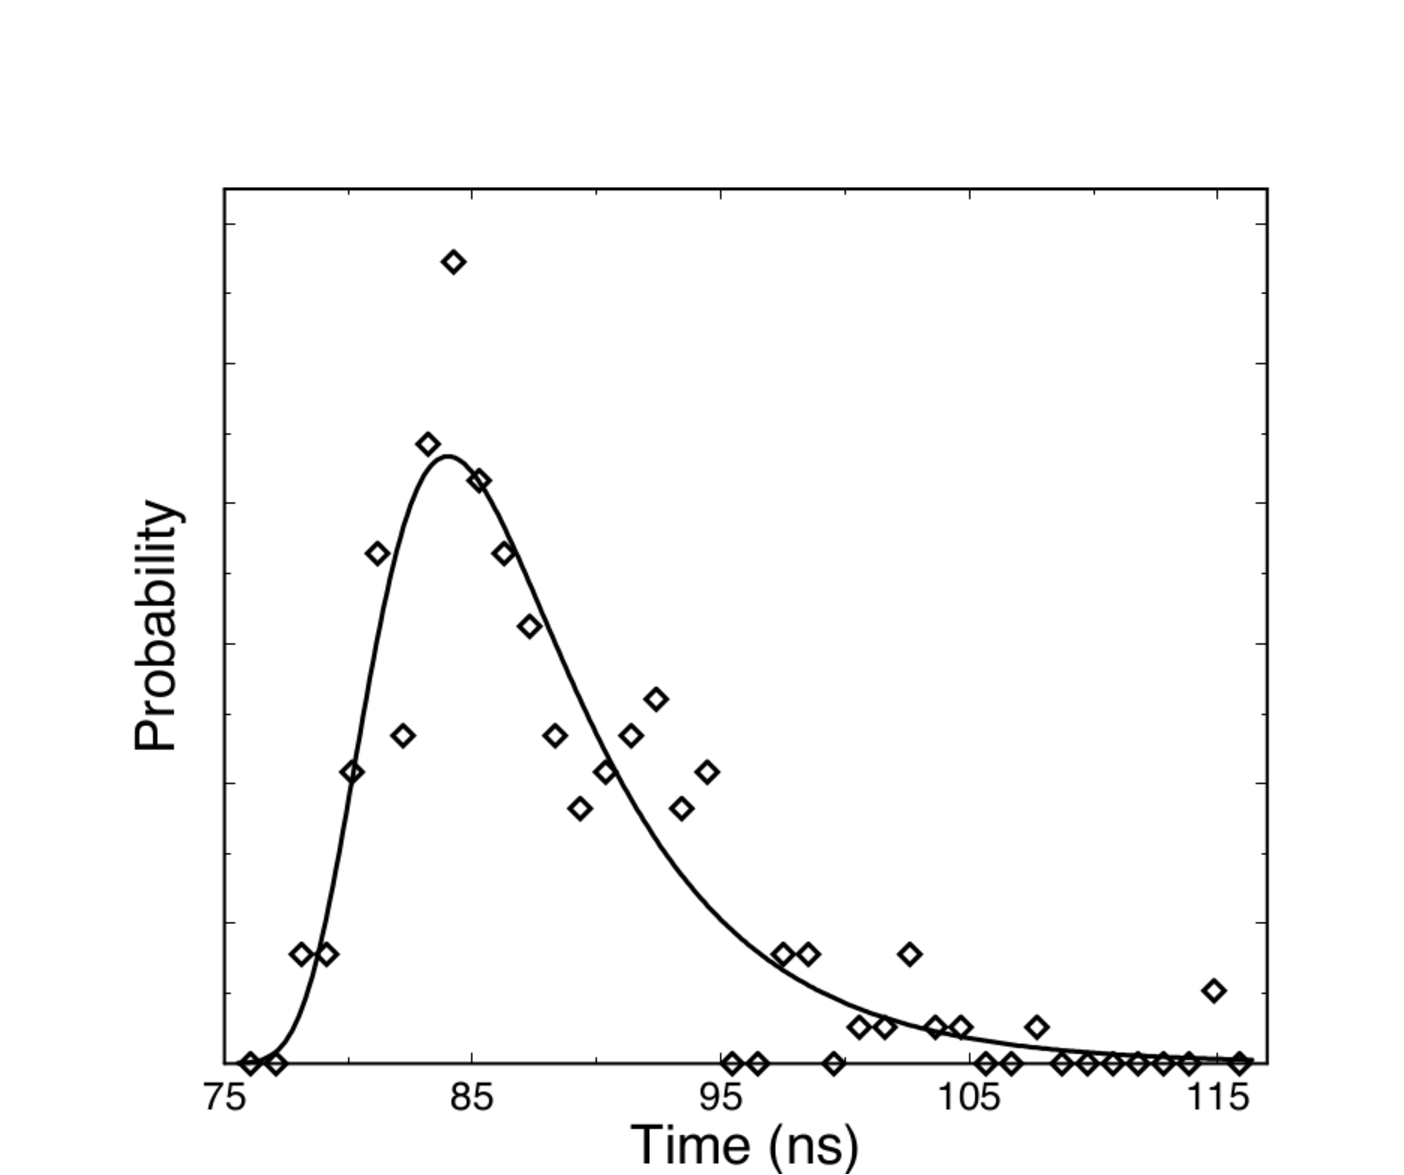
\includegraphics[width=0.3\textwidth]{./graficos/fig_9Vis.pdf}

\includegraphics[width=0.3\textwidth]{./graficos/ciclista.png}
\caption{Caption general}
\label{figGeneral}
\end{figure}
\end{frame}
%%%%%%%%%%%%%%%%%%%%%%%%%%%%%%%%%%%%%%%%%%%%
\subsection{Uso no tan frecuente}
\begin{frame}[fragile]{Uso no tan frecuente}
Lo que no es tan conocido es que, al incorporarlos, permite editarlos ligeramente.
%\vspace{-1cm}
%
\includegraphics[angle=0, width=3cm]{./graficos/ciclista}
\begin{figure}
\centering
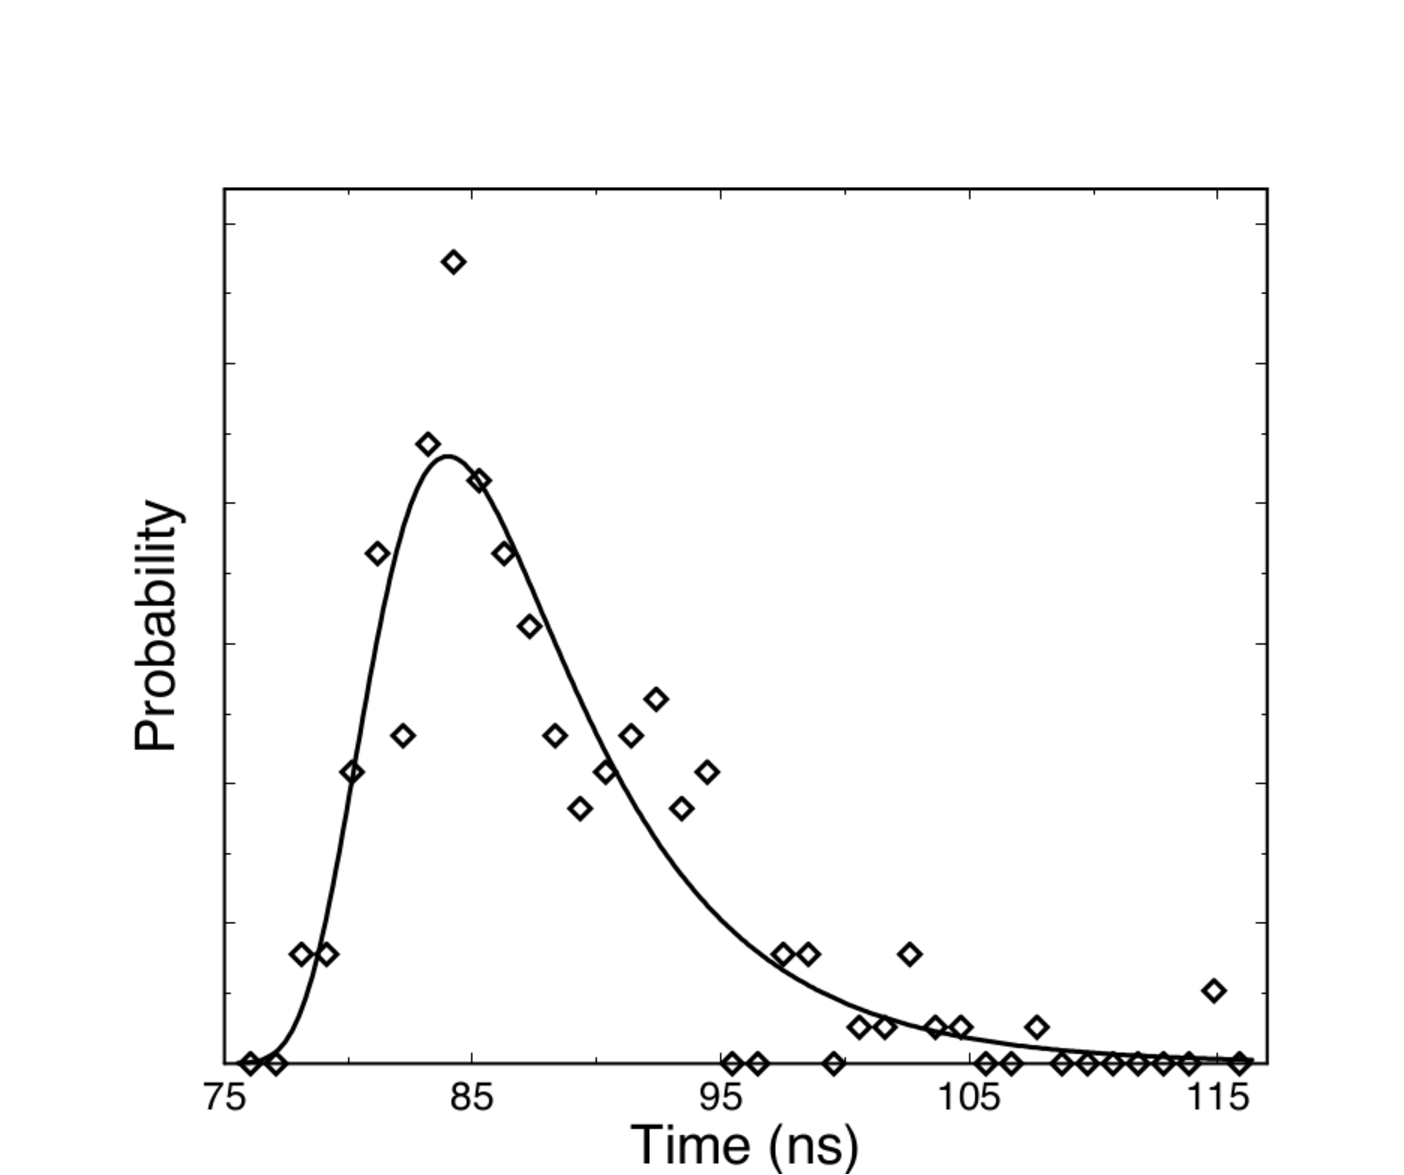
\includegraphics[width=6cm]{./graficos/fig_9Vis}
\put(-90,5){
\includegraphics[angle=-10,scale=0.4]{./graficos/ciclista}}
\caption{Redimensionar, girar y superponer imágenes}
\end{figure}
{\scriptsize OJO!  Requiere 
\href{https://docs.gimp.org/2.10/es/gimp-using-web-transparency.html}{\color{blue}fondo transparente} en la figura a superponer (objeto).}
\end{frame}
%%%%%%%%%%%%%%%%%%%%%%%%%%%%%%%%%%%%%%%%%%%%%%

\begin{frame}[fragile]{Uso no tan frecuente}
Lo que no es tan conocido es que, al incorporarlos, permite editarlos ligeramente.

\begin{figure}

\includegraphics[trim = 50mm 0mm 190mm 40mm, clip,width=4.5cm]{./graficos/sorpresa}
\hspace{-0.3cm}
\reflectbox{

\includegraphics[trim = 50mm 0mm 190mm 40mm, clip,width=4.5cm]{./graficos/sorpresa}
}
\put(-195,135){{\color{green}   \LARGE \textbf{Powered by \LaTeX}}}
\caption{Selección, simetrizar, incluir texto}
\end{figure}

\end{frame}


%%%%%%%%%%%%%%%%%%%%%%%%%%%%
\section{Inserción de gráficos}
%%%%%%%%%%%%%%%%%%%%%%%%%%%%
\subsection{Preparación del gráfico}
\begin{frame}{Generalidades sobre formatos gr\'aficos}
\begin{block}{Mapas de bits} 
\begin{center}

\includegraphics[width=7cm]{./graficos/sorpresa.jpg}
\end{center}
Extensiones: BMP, JPEG, GIF, PNG y TIFF. \\
{\small Desventaja: deformaciones al reescalar y gran tama\~no.}
\end{block}
\end{frame}
%%%%%%%%%%%%%%%%%%%%%%%%%%%%
\begin{frame}{Generalidades sobre formatos gr\'aficos}
\begin{block} {Gr\'aficos vectoriales} 
%\vspace{-1cm}
\begin{center}
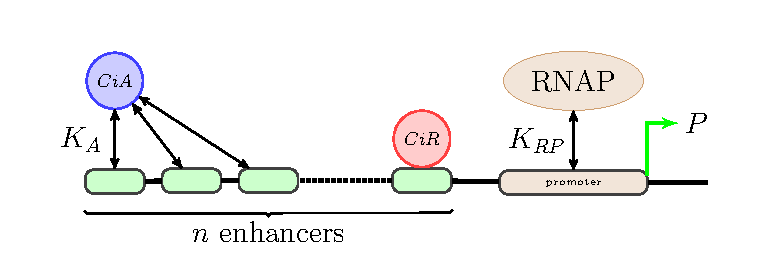
\includegraphics[width=10cm]{./graficos/bp2.pdf}
\end{center}
Extensiones: EPS, PDF, SVG, WMF \\
{\small Nota: !`Estos archivos pueden insertar mapas de bits! }
\end{block}
\end{frame}
%%%%%%%%%%%%%%%

\begin{frame}{Preparaci\'on de gr\'aficos para insertar en \LaTeX}
El formato del gr\'afico a insertar depende del compilador empleado:
\begin{enumerate}
\item \it{latex + dvips}  se requiere PS / EPS {\scriptsize(con \href{http://tex.stackexchange.com/questions/133786/no-boundingbox-error-message}{\color{blue}BoundingBox})}
\item \it {pdflatex} se requiere PNG {\scriptsize(mapas de bits simples)}, JPEG {\scriptsize(fotograf\'ias)} o PDF {\scriptsize(gr\'aficos vectoriales)}
\end{enumerate}

\vspace{0.5cm}
Esto requiere de programas espec\'ificos de transformaci\'on:
\begin{itemize}
\item {\sc EPS a PDF}: \href{http://tug.org/epstopdf/}{\color{blue}epstopdf}
%\item {\sc JPEG a EPS}: \href{http://www.pdflib.com/download/free-software/jpeg2ps/}{jpeg2ps}
\item {\sc Todo a Todo}: \href{http://www.inkscape.org/es/}{\color{blue}Inkscape}, 
\href{http://www.imagemagick.org}{\color{blue}ImageMagick} o \href{http://www.gimp.org/}{\color{blue}Gimp}
\item ........
\end{itemize}
Ver detalles en el siguiente  \href{https://w.wiki/9Luv}{\color{blue}wikibook}.
\end{frame}

%%%%%%%%%%%%%%%%%%%%%%%%%%%%%%%%%%%%%%%%%%
%\subsection{Inserción de un gr\'afico}
%%%%%%%%%%%%%%%%%%%%%
\begin{frame}[fragile]{Insertar el gr\'afico como una figura}
Declaraci\'on del paquete graphicx en el pre\'ambulo:
\begin{verbatim}\usepackage{graphicx} \end{verbatim}

Inserci\'on del gr\'afico en el documento:
\begin{verbatim}
\begin{figure}[h]
  \centering
  \includegraphics[parametros]{nombregrafico}
  \caption{Leyenda bajo el grafico}
  \label{fig:etiqueta}
\end{figure}
\end{verbatim}
Mediante los par\'ametros se puede modificar el aspecto, lo que 
nos permite editarlos ligeramente.
\end{frame}


%%%%%%%%%%%%%%%%%%%%%%%%%%%%
\section{Edición de gráficos}
%%%%%%%%%%%%%%%%%%%%%%%%%%%%

\begin{frame}[fragile]{Parámetros para modificar una figura}
Parámetros empleados más usualmente:
\begin{itemize}
    \item \verb|scale=0.5 | \hfill escala el tamaño a la mitad
    \item \verb|height=5cm | \hfill fija la altura del gráfico a 5cm
    \item \verb|width=0.5\textwidth | \hfill anchura = mitad del espacio para texto.
    \item \verb|angle=90 |\hfill  gira la imagen 90 grados.
    \item \verb|trim = 10mm 5mm 50mm 55mm, clip| \hfill Recorta la imagen quitando
\verb|trim = <left> <lower> <right> <upper> | \hfill 10mm por izda,...
    \item \verb|draft| \hfill no se incluye el gráfico pero deja el espacio apropiado.
\end{itemize}
\vspace{1cm}
Para profundizar ver documentaci\'on paquete \href{https://ctan.org/pkg/graphicx}{\color{blue} graphicx}. \\
{\scriptsize El paquete  alternativo \href{https://ctan.org/pkg/svg}{\color{blue} svg} permite incluir/editar gráficos en este formato vectorial.}
\end{frame}
%%%%%%%%%%%%%%%%%%%%%%%%%%%%%%%%%%%%%%%%%%
\begin{frame}[fragile]{Localización de la figura en el texto}
El entorno figure es flotante, esto es, \LaTeX{} ``decide''
dónde lo pone. Si queremos controlar este proceso tenemos varias 
opciones:
\begin{itemize}
    \item Control débil del entorno \verb|figure| con parámetros 
    de control h, b, t. 
    \item Empleo del entorno \verb|wrapfigure| gracias al paquete \href{https://www.ctan.org/pkg/wrapfig}{\color{blue} wrapfig}.
    \item Empleo del parámetro H del paquete \href{https://www.ctan.org/pkg/float}{\color{blue} float}.
    \item Usar \verb|includegraphics| sin entorno \verb|figure|. \hfill (No recomendable)
\end{itemize}
\vspace{1cm}
Ver detalles en \href{https://www.overleaf.com/learn/latex/Positioning_images_and_tables}{\color{blue}ayuda de OverLeaf}.
\end{frame}

%%%%%%%%%%%%%%%%%%%%%%%%%%%%%%%%%%%%%%%%%%
\begin{frame}[fragile]{Espacio entre la figura y el texto}
Es posible que al insertar un gráfico quede mucho espacio entre
el texto y el gráfico.  Para comprobarlo usar el comando frame
\begin{wrapfigure}{r}{4cm}
\frame{
\includegraphics[width=3.cm]{./graficos/ciclista.jpeg}}
\end{wrapfigure}
\begin{verbatim}
\begin{figure}[h]
\frame{
\includegraphics{file}
}
\end{figure}
\end{verbatim}




\end{frame}

%%%%%%%%%%%%%%%%%%%%%%%%%%%%

\begin{frame}[fragile]{Espacio entre la figura y el texto}
y posteriormente recortar con \verb| trim | y \verb| clip|
%\only<1>{
\begin{wrapfigure}{r}{4cm}
\vspace{2cm}
\frame{
\includegraphics[trim = 12mm 15mm 9mm 9mm, clip,width=3.cm]{./graficos/ciclista.jpeg}}
\end{wrapfigure}
\begin{verbatim}
\begin{figure}[h]
\frame{
\includegraphics[trim = 12mm 15mm 9mm 9mm, clip]{file}
}
\end{figure}
\end{verbatim}
\end{frame}




%%%%%%%%%%%%%%%%%%%%%%%%%%%%
\begin{frame}[fragile]{Otra utilidad: inclusión páginas completas pdf}
\vspace{-4cm}
\begin{wrapfigure}{r}{6cm}
\hspace{0.5cm}

\includegraphics[width=5.cm]{./graficos/DeclaraciondeOriginalidadTFG.pdf}
\end{wrapfigure}
\vspace{1cm}
El paquete \href{https://ctan.org/pkg/pdfpages}{\color{blue}pdfpages} permite incluir páginas seleccionadas de un pdf en un documento \LaTeX{}. 

{\scriptsize Utilidad: generar documentación acreditativa, \\incluir declaraciones en documentos, etc...}

\begin{verbatim}
\includepdf[]{file.pdf}
\end{verbatim}
\end{frame}




%%%%%%%%%%%%%%%%%%%%%%%%%%%%%%
\begin{frame}[fragile]{Uso avanzado: sitios de interés}
Puesto que es imposible mostrar paquetes de interés para una 
audiencia heterogénea lo mejor es mostrar dónde y cómo localizarlos

\href{https://www.ctan.org}{\color{blue}https://www.ctan.org}

%\href{https://github.com/pgf-tikz/pgf}{\color{blue}https://github.com/pgf-tikz/pgf}

\href{https://es.wikibooks.org/wiki/Manual_de_LaTeX/Inclusión_de_gráficos/Gráficos_con_TikZ}{\color{blue}Wikibooks: Gráficos con Tikz}

%\href{http://www.texample.net/tikz/examples/}{\color{blue}http://www.texample.net/tikz/examples/}

%\href{https://tex.stackexchange.com/questions/42611/list-of-available-tikz-libraries-with-a-short-introduction}{\color{blue} Librerías de Tikz}

\end{frame}


%%%%%%%%%%%%%%%%%%%%%%%%%%%%%%%%%%%%%%%
%\begin{frame}[allowframebreaks]{Referencias}
%\bibliography{presentacion}
%%\bibliographystyle{abbrv}
%\end{frame}
%
\end{document}
